%%
% This is an Overleaf template for presentations
% using the TUM Corporate Desing https://www.tum.de/cd
%
% For further details on how to use the template, take a look at our
% GitLab repository and browse through our test documents
% https://gitlab.lrz.de/latex4ei/tum-templates.
%
% The tumbeamer class is based on the beamer class.
% If you need further customization please consult the beamer class guide
% https://ctan.org/pkg/beamer.
% Additional class options are passed down to the base class.
%
% If you encounter any bugs or undesired behaviour, please raise an issue
% in our GitLab repository
% https://gitlab.lrz.de/latex4ei/tum-templates/issues
% and provide a description and minimal working example of your problem.
%%

%\makeatletter
%\def\input@path{{../beamer/}}
%\makeatother

\documentclass[
  german,            % define the document language (english, german)
  aspectratio=169,    % define the aspect ratio (169, 43)
  % handout=2on1,       % create handout with multiple slides (2on1, 4on1)
  % partpage=false,     % insert page at beginning of parts (true, false)
  % sectionpage=true,   % insert page at beginning of sections (true, false)
]{tumbeamer}


% load additional packages
\usepackage{booktabs}
\usepackage{graphicx}
\usepackage{tikz}
\usepackage{url}
\usepackage{pgfplots}
\usepackage{hyperref}
\usepackage{pmboxdraw}
\usepackage{float}
\usepackage{listings}
\usepackage{circuitikz}
%\usepackage[european]{circuitikz}

% image path
\graphicspath{ {./resources/} }

% presentation metadata
\title{Übung 14: Fragestunde}
\subtitle{Einführung in die Rechnerarchitektur}
\author{Niklas Ladurner}

\institute{\theChairName\\\theDepartmentName\\\theUniversityName}
\date[\today]{\today}

\footline{\insertauthor~|~\insertshorttitle~|~\insertshortdate}


% macro to configure the style of the presentation
\TUMbeamersetup{
  title page = TUM tower,         % style of the title page
  part page = TUM toc,            % style of part pages
  section page = TUM toc,         % style of section pages
  content page = TUM more space,  % style of normal content pages
  tower scale = 1.0,              % scaling factor of TUM tower (if used)
  headline = TUM threeliner,      % which variation of headline to use
  footline = TUM default,         % which variation of footline to use
  % configure on which pages headlines and footlines should be printed
  headline on = {title page},
  footline on = {every page, title page=false},
}

% available frame styles for title page, part page, and section page:
% TUM default, TUM tower, TUM centered,
% TUM blue default, TUM blue tower, TUM blue centered,
% TUM shaded default, TUM shaded tower, TUM shaded centered,
% TUM flags
%
% additional frame styles for part page and section page:
% TUM toc
%
% available frame styles for content pages:
% TUM default, TUM more space
%
% available headline options:
% TUM empty, TUM oneliner, TUM twoliner, TUM threeliner, TUM logothreeliner
%
% available footline options:
% TUM empty, TUM default, TUM infoline


\begin{document}

\maketitle

\begin{frame}[c]{}{}
  \begin{center}
    \LARGE  Durchzählen!
  \end{center}
\end{frame}

\begin{frame}[fragile, c]{Material aus den Tutorübungen}{}
  \begin{itemize}
    \item Ihr dürft gerne meine Slides/Mitschriften aus den Tutorien mit 
    euren Kommilitonen teilen
    \item Bitte keine Weitergabe von Dokumenten, sondern Verweis/Links zur Website (home.in.tum.de/~ladu/), 
    ermöglicht mir evtl. Fehler auszubessern
    \item \underline{KEIN UPLOAD} auf Studocu/Studydrive oder sonst irgendwo
  \end{itemize}
\end{frame}

\begin{frame}[fragile, c]{Klausur}{}
\begin{itemize}
  \item Student Card nicht vergessen
  \item Genügend Kugelschreiber mitnehmen, kein Rot/Grün/Bleistift
  \item Essen/Trinken ist auch erlaubt solange ihr damit niemanden stört
  \item in die Endterm zu gehen lohnt sich immer, leer abgeben ist auch eine Möglichkeit
\end{itemize}
\end{frame}


\begin{frame}[fragile, c]{Statistik zur Endterm WS 22/23}{}
  \begin{tikzpicture}[remember picture,overlay]
    \node[inner sep=0pt, outer sep=40pt, anchor=north west] at ([xshift=-1cm]current page.north west) {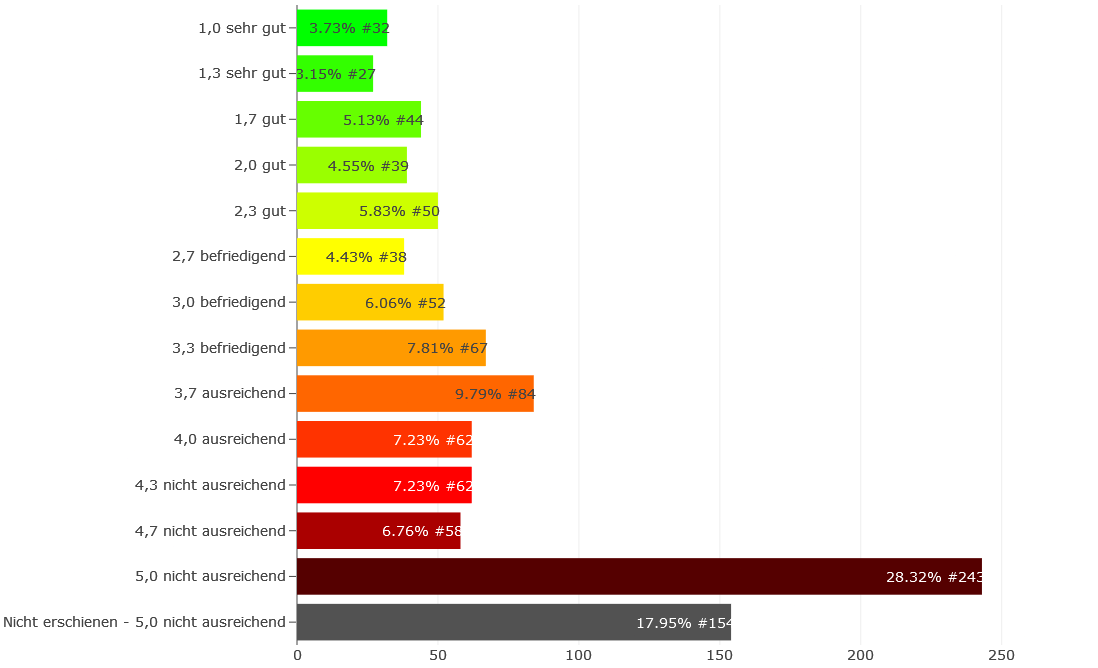
\includegraphics[height=0.85\textheight]{w14_endterm.png}};
  \end{tikzpicture}

  \begin{columns}[c]
    \begin{column}{0.5\textwidth}
    \end{column}
    \begin{column}{0.5\textwidth}
      \begin{itemize}
        \item Angetreten: 1012
        \item Antritt zählt: 858
        \item Anteil negativer Beurteilungen: 42.31\%
        \item Durchschnitt gesamt: 3.65
        \item Durchschnitt bestanden: 2.77
      \end{itemize}
    \end{column}
  \end{columns}
\end{frame}

\begin{frame}[fragile, c]{Statistik zur Retake WS 22/23}{}
  \begin{tikzpicture}[remember picture,overlay]
    \node[inner sep=0pt, outer sep=40pt, anchor=north west] at ([xshift=-1cm]current page.north west) {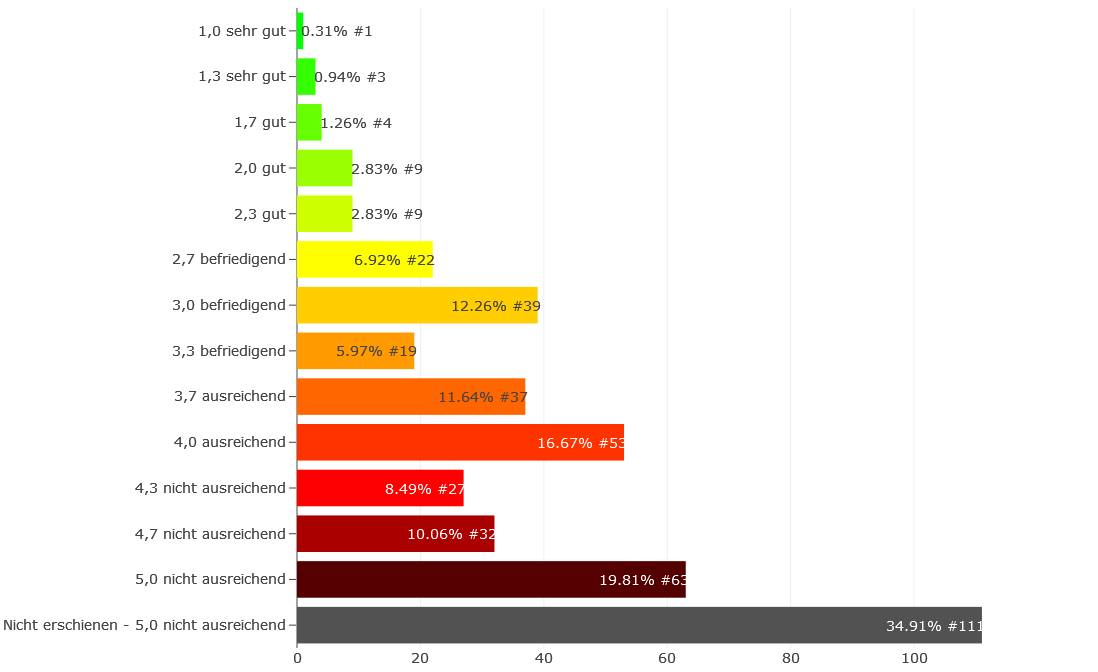
\includegraphics[height=0.85\textheight]{w14_retake.png}};
  \end{tikzpicture}

  \begin{columns}[c]
    \begin{column}{0.5\textwidth}
    \end{column}
    \begin{column}{0.5\textwidth}
      \begin{itemize}
        \item Angetreten: 429
        \item Antritt zählt: 318
        \item Anteil negativer Beurteilungen: 38.36\%
        \item Durchschnitt gesamt: 3.84
        \item Durchschnitt bestanden: 3.26
      \end{itemize}
    \end{column}
  \end{columns}
\end{frame}

\begin{frame}[c]{}{}
  \begin{center}
    \LARGE Fragen?
  \end{center}
\end{frame}


\begin{frame}[c]{}{}
  \begin{center}
    \LARGE Viel Erfolg bei der Klausur :)
  \end{center}
\end{frame}

\maketitle

\end{document}
